\section{Simulation}\label{app:simulations}

\subsection{Logic}

In the model developed in Section \ref{sec:model}, there are two important assumptions underlying its basic intuition. First, the total value that can be captured by successful firms is independent of the number of successful firms - meaning the total profit from successful experiments by independent firms stays constant. Specifically, a firm with two successful experiments earns the same payoff as if it had only one successful experiment. This implies that competition among successful firms does not dissipate rents but merely distributes the total payoff in some fashion. The second assumption is that the validity of approaches is uncertain. Firms choosing the same approach are more likely to succeed or fail together than firms choosing different approaches, meaning value diversion is more likely when firms choose the same approach. In other words, firms choosing the same approach have correlated outcomes, whose effect is not fully integrated into individual firms' decisions. However, this correlation arises only if $\pi \neq 1$; if $\pi = 1$, the probability of success depends solely on implementation. Thus, firms will choose the approach with which they have the highest probability of implementation success. Target diversity at the market level would simply reflect differences in implementation ability for different approaches.

Generalizing beyond two approaches and two possible experiments to multiple approaches and multiple firms involves considerations of competition and order of entry into experimentation. While this is not analytically tractable, simulations permit us to explore the robustness of the model's intuition. We use Monte Carlo simulations to generalize the results of our model. In the baseline simulation, we define a pool of 50 firms, of which $\phi \in[0,1]$ have a high cost of experimenting (and $1-\phi$ incur a low cost). In each period, a firm is randomly selected and can choose to experiment. Firms experiment with the approach that returns the largest non-negative expected payoff and do not enter if all expected payoffs are negative. This payoff depends on the ongoing experiments and whether the firm has an ongoing experiment. Once a firm has entered twice we remove them from the pool of firms. We run simulations for different shares $\phi$ to exogenously create variation in the share of firms that enter with two experiments (a higher share of high-cost firms leads to fewer firms entering with two experiments). A simulation ends when the first low-cost firm chooses not to enter since this indicates that there will be no more entry (high-cost firms are less likely to enter than low-cost firms, given their higher cost). We run 400 simulations for $\phi = \{0, 0.1, 0.2, 0.3, 0.4, 0.5, 0.6, 0.7, 0.8, 0.9, 1\}$

Figure \ref{fig:simulations} presents results from the baseline simulation, where we simulate firms choosing between two approaches, $a$ and $b$, where $\pi_a < \pi_b$. Firms continue to enter until they become unprofitable with either approach. In panel \ref{subfig:sims_choice}, we link the market-level share of multi-experiment firms to the diversity of approaches used. Maximum diversity would be an even split between approach $a$ and $b$, with target diversity defined as one minus the share of experiments using approach $a$. Our simulations support the analytical prediction that greater approach diversity occurs when firms conduct multiple experiments on average. In panels \ref{subfig:sims_success_share} and \ref{subfig:sims_choice_to_outcomes}, we show results from simulations predicted by Propositions \ref{prop:model-outcomes} and \ref{prop:atleastone}. Markets with a greater share of multi-experiment firms have a lower individual experiment success rate. However, in markets with greater approach diversity---associated with more multi-experiment firms---we observe a higher probability of at least one experiment succeeding.

\begin{lightfigure}[h!]
\caption{\textsc{Simulation Results}}
\label{fig:simulations}
    \centering
    \begin{sublightfigure}[t]{.3\textwidth}
        \centering
        \caption{}
        \includegraphics[width=\linewidth]{figures/sims_choice.pdf}
        \label{subfig:sims_choice}
    \end{sublightfigure}
    \begin{sublightfigure}[t]{.3\textwidth}
        \centering
        \caption{}
        \includegraphics[width=\linewidth]{figures/sims_success_share.pdf}
        \label{subfig:sims_success_share}
    \end{sublightfigure}
    \begin{sublightfigure}[t]{.3\textwidth}
        \centering
        \caption{}
        \includegraphics[width=\linewidth]{figures/sims_choice_to_atleastone_successe.pdf}
        \label{subfig:sims_choice_to_outcomes}
    \end{sublightfigure}
\caption*{\scriptsize\emph{Notes:} These figures report binned scatter plots of our simulation results, illustrating the relationships predicted by each proposition. We simulate 1500 markets, creating variation in the share of large-scale experimenters by exogenously shifting the share of firms that have a high cost of experimenting. A detailed explanation of the simulation logic is provided in Appendix \ref{app:simulations}. This simulation uses the following parameters: $\pi_a = 0.4$, $\pi_b = 0.2$, $p_a = p_b = 0.3$.}
\end{lightfigure}

\subsection{Extension: Discovery of new Approaches}

A feature of our empirical context is that new approaches are discovered. Additionally, in practice, more than two approaches will be available to the experimenter. In our empirical context, for example, the average number of targets observed in a therapeutic class--year is 9.09 (median=5, std.dev.=14.21, min=2, max=210. Here, we extend our simulation framework to allow for discovery and, thus, multiple approaches. 

The logic for these simulations is identical to that deribed in the baseline simulations, but we make the following changes to introduce discovery. In each period, a new approach is discovered with probability $\gamma$. In the case of discovery, a new entrant enters with the approach, and the approach enters the domain of available approaches that subsequent experiments can choose from. We keep all parameter values the same as the baseline simulation (i.e., $\pi_a=0.4; \pi_b=0.2; p_a=p_b=0.3 $). All new approaches $k$ have a lower viability probability $\pi_k = 0.1$, but the same implementation probability $p_k = 0.3$ as existing approaches $a$ and $b$. We assume that only new entrants discover new targets and that this is their only experiment. This is to match our empirical finding, that the introduction of new approaches is more likely to happen with single-experiment firms. Keeping all other parameters constant, we vary the probability of discovery and observe the effect of discovery on the diversity of targets and success. We run 400 simulations for each combination of high-cost experimenter share $\phi = \{0, 0.2, 0.4, 0.6, 0.8, 1\}$ and discovery probability $\gamma = \{0, 0.05, 0.1\}$.

\begin{lightfigure}[h!]
    \caption{Simulating the Effect of Discovery on the Diversity of Approaches and the Outcomes of Experiments}
    \label{fig:appendix_sim_discovery_diversity}
    \centering
    \begin{sublightfigure}[t]{.3\textwidth}
        \centering
        \caption{}
        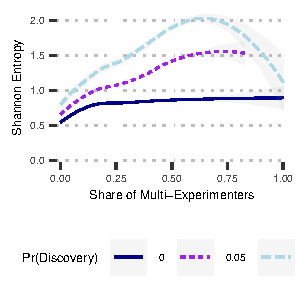
\includegraphics[width=\linewidth]{figures/sim_discovery_shannon.pdf}
        \label{subfig:target_diversity_rob1}
    \end{sublightfigure}
    \begin{sublightfigure}[t]{.3\textwidth}
        \centering
        \caption{}
        \includegraphics[width=\linewidth]{figures/sim_discovery_alo_es.pdf}
        \label{subfig:target_diversity_rob1}
    \end{sublightfigure}
    \begin{sublightfigure}[t]{.3\textwidth}
        \centering
        \caption{}
        \includegraphics[width=\linewidth]{figures/sim_discovery_alo_div.pdf}
        \label{subfig:target_diversity_rob1}
    \end{sublightfigure}
    \begin{sublightfigure}[t]{.3\textwidth}
        \centering
        \caption{}
        \includegraphics[width=\linewidth]{figures/sim_discovery_ss_es.pdf}
        \label{subfig:target_diversity_rob1}
    \end{sublightfigure}
    \begin{sublightfigure}[t]{.3\textwidth}
        \centering
        \caption{}
        \includegraphics[width=\linewidth]{figures/sim_discovery_ss_div.pdf}
        \label{subfig:target_diversity_rob1}
    \end{sublightfigure}
% \caption*{\scriptsize\emph{Notes:} }
\end{lightfigure}



In Figure \ref{fig:appendix_sim_discovery_diversity}, we report simulation results grouped by each discovery probability. In each plot we show binned scatter plots, with 50 bins. We measure the diversity of approaches with Shannon entropy, consistent with our empirical method. In panel (a), our simulations show that the probability of discovery positively moderates the relationship between the share of multi-experimenters and the diversity of approaches. In other words, for a fixed share of multi-experiment firms, when the likelihood of a new approach being discovered is higher, our simulations predict a greater diversity of approaches.

Turning to outcomes, the results are less clear-cut. In panels (b) and (c), we look at the probability of at least one success, and in panels (d) and (e), we look at the average success rate. In panel (b), the simulations suggest a small benefit from discovery on the probability of at least one success. This is consistent with our previous results: a higher discovery rate is associated with a greater diversity of approaches, which is associated with a higher probability of the market finding at least one success. Panel (c) is harder to interpret, but our results suggest a declining benefit to higher discovery rates. Holding the diversity of approaches constant, a higher probability of at least one success is achieved when the discovery rate is lower. 

Panel (d) also conforms with prior results. The share of successful experiments is lower when a market consists of a greater share of multi-experiment firms, especially when the discovery rate is higher. Discovery leads to new approaches becoming available, but individually, they have a smaller probability of success. Panel (e) suggests results consistent with the intuition of the panel (c). Holding the diversity of approaches constant, the share of experimental successes will be lower when the discovery rate is higher.






% \subsection{Extension: Rent Dissipation}


% \begin{lightfigure}[h!]
% \caption{\textsc{Simulating the Effect of Rent Dissipation on the Diversity of Approaches and the Outcomes of Experiments}}
% \label{}
%     \centering
%     \begin{sublightfigure}[t]{.3\textwidth}
%         \centering
%         \caption{}
%         \includegraphics[width=\linewidth]{figures/sim_rentdiss_diversity.pdf}
%         \label{subfig:sim_rentdiss_diversity}
%     \end{sublightfigure}
%     \begin{sublightfigure}[t]{.3\textwidth}
%         \centering
%         \caption{}
%         \includegraphics[width=\linewidth]{figures/sim_rentdiss_success_share.pdf}
%         \label{subfig:sim_rentdiss_success_share}
%     \end{sublightfigure}
%     \begin{sublightfigure}[t]{.3\textwidth}
%         \centering
%         \caption{}
%         \includegraphics[width=\linewidth]{figures/sim_rentdiss_atleastone_on_share.pdf}
%         \label{subfig:sim_rentdiss_atleastone_on_share}
%     \end{sublightfigure}
% \caption*{\scriptsize\emph{Notes:} 
% This simulation uses the following parameters: $\pi_a = 0.4$, $\pi_b = 0.2$, $p_a = p_b = 0.3$.}
% \end{lightfigure}


% \subsection{Extension: Value of Experimentation}

% \begin{lightfigure}[h!]
% \caption{\textsc{Simulating the Effect of Value on the Diversity of Approaches and the Outcomes of Experiments}}
% \label{}
%     \centering
%     \begin{sublightfigure}[t]{.3\textwidth}
%         \centering
%         \caption{}
%         \includegraphics[width=\linewidth]{figures/value_sims_diversity.pdf}
%         \label{subfig:value_sims_diversity}
%     \end{sublightfigure}
%     \begin{sublightfigure}[t]{.3\textwidth}
%         \centering
%         \caption{}
%         \includegraphics[width=\linewidth]{figures/value_sims_success_share.pdf}
%         \label{subfig:value_sims_success_share}
%     \end{sublightfigure}
%     \begin{sublightfigure}[t]{.3\textwidth}
%         \centering
%         \caption{}
%         \includegraphics[width=\linewidth]{figures/value_sims_atleastone_success.pdf}
%         \label{subfig:value_sims_atleastone_success}
%     \end{sublightfigure}
% \caption*{\scriptsize\emph{Notes:} 

% This simulation uses the following parameters: $\pi_a = 0.4$, $\pi_b = 0.2$, $p_a = p_b = 0.3$.}
% \end{lightfigure}
